\chapter{Introduction}
While approaching a more and more ubiquitous network experience where we are
connected to different personal area networks (PAN) or even the global internet
around the clock two problems become more important. One problem is the power
consumptions of devices that makes the ubiquity possible. In contrast to other
computing device we want them to be well hidden and don't disturb us. Changing
batteries or having power cables around is not a real option for them. On the
other hand wireless communication protocols with 802.11 as the leading option
are a good choice for mobile devices like notebooks or smartphones but are still
to power consuming for such small ubiquitous devices. With 802.15.4 a new
protocol was designed for exactly such small, power constraint devices. We will
use it in our research and have some more informations about it prepared
in~\ref{intro802154}.

The second problem is disrupted network connection be it due to movement or
similar. The most widely used protocol family with IP, UDP, TCP and more is not
designed for disrupted networks. They expect a working physical connection below
them to work as expected. If this is not the case the packets may be just lost
as in case of UDP or have to be re-transmitted. This re-transmission could be
problematic if the network connection is more often unavailable then available.
For such scenarios delay tolerant networking was designed to send to the
packets, perhaps over several hopes, to the destination without needing to
establish a channel between source and destination. In~\ref{introdtn} we give a
short introduction into DTN before describing our convergence layer
in~\ref{802154layer}.

\section{IEEE 802.15.4}
\label{intro802154}
Driven by an IEEE working group the 802.15.4 standard provides the physical and
mac access control layer for so called low-rate wireless personal area network
(LR-WPAN). The emphasis is on low cost devices for communication without
infrastructure in a nearby environment. The communication range would be up to
10m and offers nowadays a transfer rate up to 250 kbit/s. The standard specifies
three possible frequency bands to operate in. The usage of some may be
restricted in different countries but one band is available worldwide. Other
features of 802.15.4 includes collision avoidance through CSMA/CA, build in
support for secure communication through cryptography, power management through
link quality control and energy detection as well as reserved time slots for
real-time operations.

As already covered the standard does only cover the two lowest layer of a
protocol stack. Supplement it to a fully functional networking stack is the aim
of different other specifications as shown in figure~\ref{fig:802154layer}. The
most famous would be ZigBee. With 6LowPAN there is also work underway to link
LR-WPAN together with standard internet protocols like IPv6.

Specified for an infrastructure-less network the topologies may be star or
Peer-to-Peer based as well a composition of both. \ref{fig:802154topologies}
shows how an example star network topology could look as well as a Peer-to-Peer
topology. Two different device types are allowed. full-function device (FFD) and
reduced-function device (RFD). The RFD is a really simple device which can only
connect to one FFD at a time. Therefor it can only act as a leaf in all
described topologies. In contrast the FFD is able to act as a coordinator to
span up a whole PAN and rely messages to other nodes. At least one coordinator
is needed in every network. One thing to keep in mind is that routing is not
covered by the standard. To rely messages over different hops the supplement
upper layers need to take care of this.

\begin{figure}
  \begin{center}
    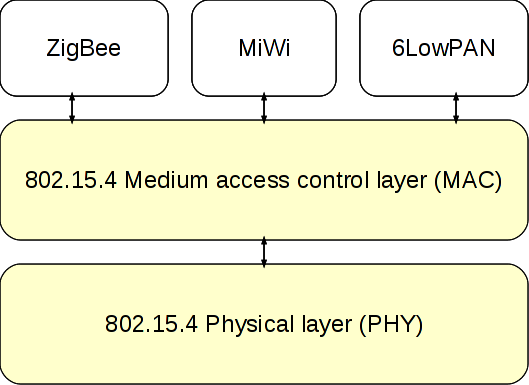
\includegraphics[height=6cm]{images/802154layer}
    \caption{IEEE 802.15.4 lower layers with optional upper layers}
        \label{fig:802154layer}
  \end{center}
\end{figure}

\begin{figure}
  \begin{center}
    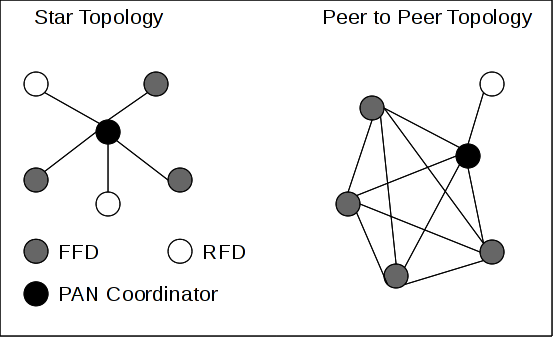
\includegraphics[height=6cm]{images/802154topology}
    \caption{IEEE 802.15.4 network topologies}
        \label{fig:802154topologies}
  \end{center}
\end{figure}

\section{DTN}
\label{introdtn}
Delay-tolerant networking is the other core technology that is used within this
thesis. The need for communication between nodes without continuous network
connectivity is what DTN seeks to address. Most modern routing protocols only
send out the real data once a complete route to the destination is established.
A communication over such an approach is only possible if source and destination
are long enough within a connected network to establish a route between them,
transfer the data and maybe acknowledge the transfer.

DTN in contrast uses a store and forward approach which sends out the data
directly together with the destination address. The bundle protocol in
\cite{RFC5050} was specified for this. One approach to maximize the probability
of a successful delivered message would be to send out multiple copies of the
same message, maybe to different hops. Such an approach obviously increases the
network and storage load and may not be useful for constrained devices like
sensor nodes.

The bundle protocol specifies an overlay network which interacts with the lower
layers over bundle convergence layers. The lower layers are not bound to be IP
based even if that is the one widely used. In this thesis we describe the usage
of the DTN implementation IBR-DTN over a 802.15.4 radio link on a linux based
system.
